% Auto-generated by plot_benchmarks.py
% Histogram figures (time & memory) per matrix size

\begin{figure}[H]
  \centering
  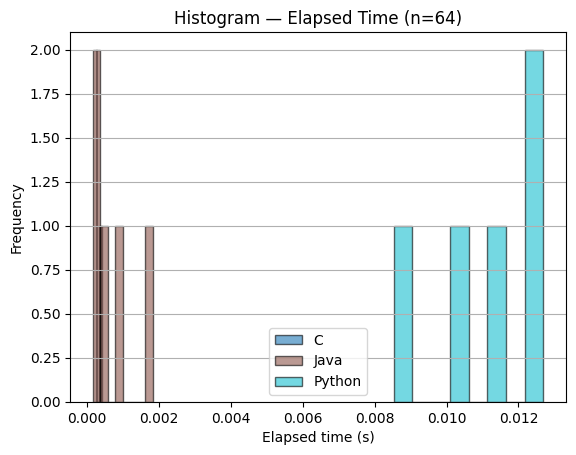
\includegraphics[width=.75\linewidth]{hist_time_n64.png}
  \caption{Histogram of elapsed time by language ($n=64$).}
\end{figure}

\begin{figure}[H]
  \centering
  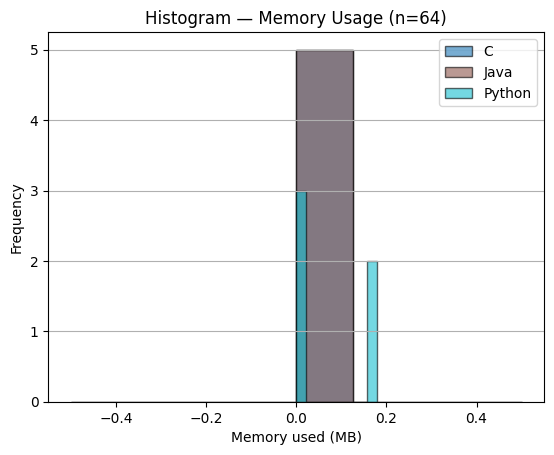
\includegraphics[width=.75\linewidth]{hist_mem_n64.png}
  \caption{Histogram of memory usage by language ($n=64$).}
\end{figure}

\begin{figure}[H]
  \centering
  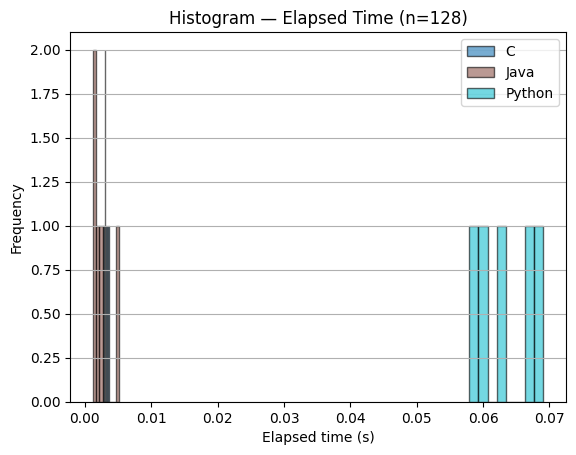
\includegraphics[width=.75\linewidth]{hist_time_n128.png}
  \caption{Histogram of elapsed time by language ($n=128$).}
\end{figure}

\begin{figure}[H]
  \centering
  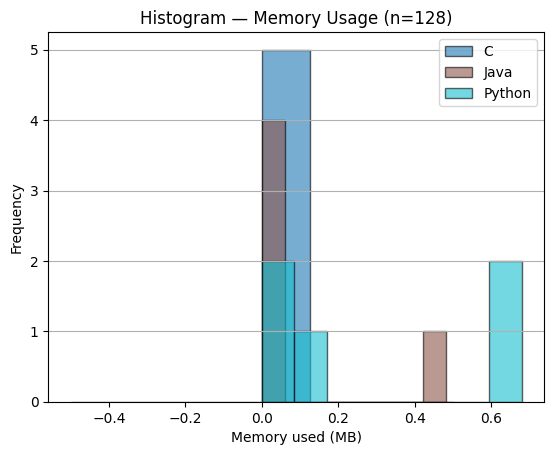
\includegraphics[width=.75\linewidth]{hist_mem_n128.png}
  \caption{Histogram of memory usage by language ($n=128$).}
\end{figure}

\begin{figure}[H]
  \centering
  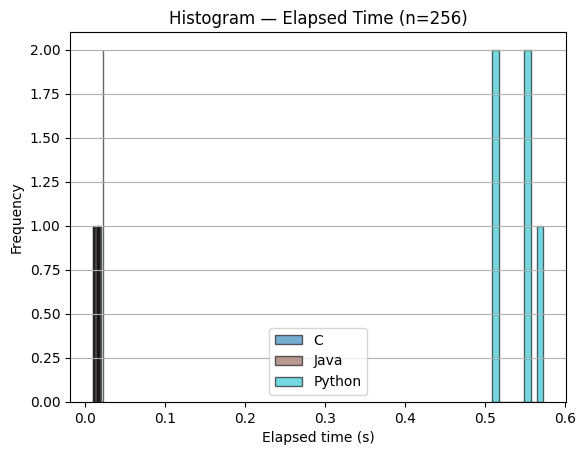
\includegraphics[width=.75\linewidth]{hist_time_n256.png}
  \caption{Histogram of elapsed time by language ($n=256$).}
\end{figure}

\begin{figure}[H]
  \centering
  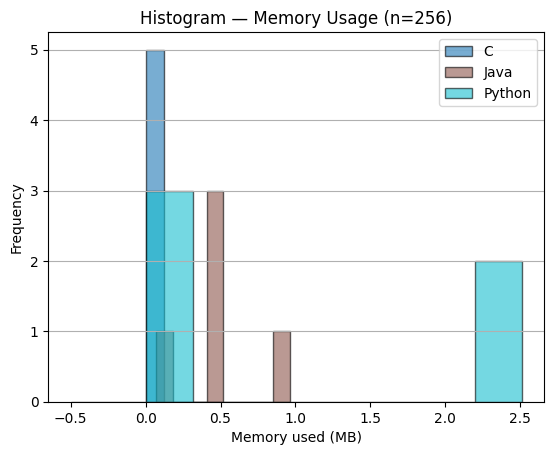
\includegraphics[width=.75\linewidth]{hist_mem_n256.png}
  \caption{Histogram of memory usage by language ($n=256$).}
\end{figure}

\begin{figure}[H]
  \centering
  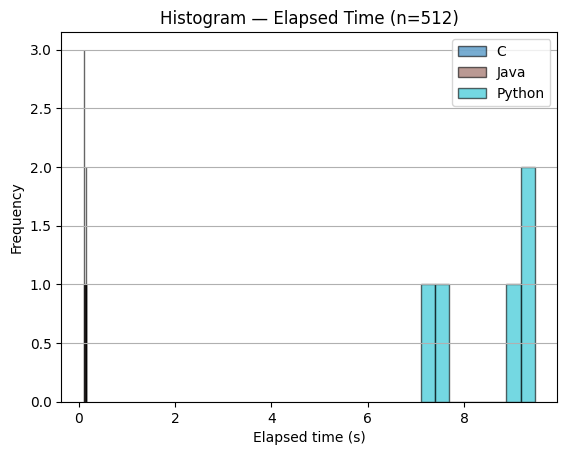
\includegraphics[width=.75\linewidth]{hist_time_n512.png}
  \caption{Histogram of elapsed time by language ($n=512$).}
\end{figure}

\begin{figure}[H]
  \centering
  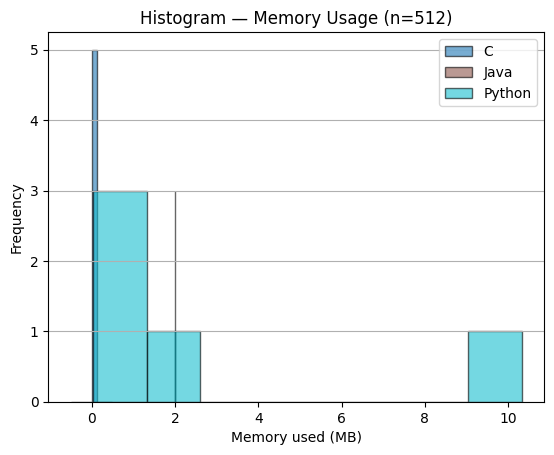
\includegraphics[width=.75\linewidth]{hist_mem_n512.png}
  \caption{Histogram of memory usage by language ($n=512$).}
\end{figure}

\begin{figure}[H]
  \centering
  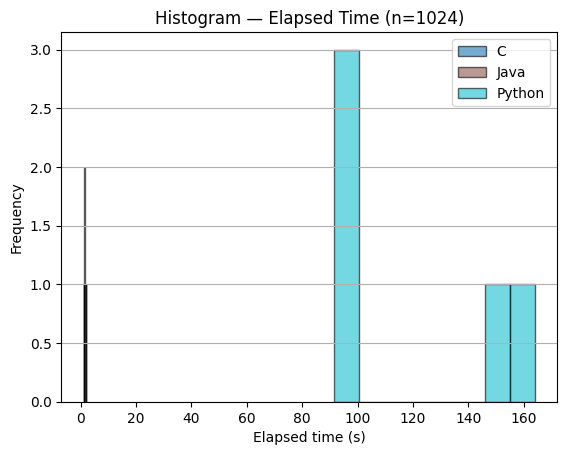
\includegraphics[width=.75\linewidth]{hist_time_n1024.png}
  \caption{Histogram of elapsed time by language ($n=1024$).}
\end{figure}

\begin{figure}[H]
  \centering
  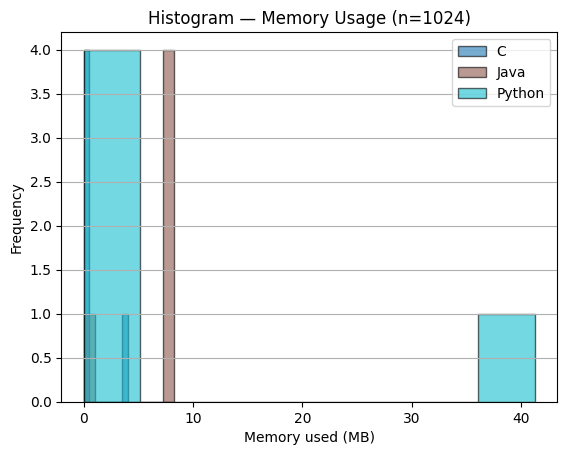
\includegraphics[width=.75\linewidth]{hist_mem_n1024.png}
  \caption{Histogram of memory usage by language ($n=1024$).}
\end{figure}
